%%%%%%%%%%%%%%%%%%%%%%%%%%%%%%%%%%%%%%%%%
% University Assignment Title Page 
% LaTeX Template
% Version 1.0 (27/12/12)
%
% This template has been downloaded from:
% http://www.LaTeXTemplates.com
%
% Original author:
% WikiBooks (http://en.wikibooks.org/wiki/LaTeX/Title_Creation)
%
% License:
% CC BY-NC-SA 3.0 (http://creativecommons.org/licenses/by-nc-sa/3.0/)
% 
% Instructions for using this template:
% This title page is capable of being compiled as is. This is not useful for 
% including it in another document. To do this, you have two options: 
%
% 1) Copy/paste everything between \begin{document} and \end{document} 
% starting at \begin{titlepage} and paste this into another LaTeX file where you 
% want your title page.
% OR
% 2) Remove everything outside the \begin{titlepage} and \end{titlepage} and 
% move this file to the same directory as the LaTeX file you wish to add it to. 
% Then add \input{./title_page_1.tex} to your LaTeX file where you want your
% title page.
%
%%%%%%%%%%%%%%%%%%%%%%%%%%%%%%%%%%%%%%%%%

%----------------------------------------------------------------------------------------
%	PACKAGES AND OTHER DOCUMENT CONFIGURATIONS
%----------------------------------------------------------------------------------------

\documentclass[12pt]{article}
\usepackage[utf8]{inputenc}
\usepackage[french]{babel}
\usepackage{bold-extra}
\usepackage{lmodern,textcomp}


%\usepackage{hyperref}

%% BIBTEX %%
\usepackage[backend=biber, sorting=none, style=numeric, natbib=true]{biblatex}
\DeclareCiteCommand{\supercite}[\mkbibsuperscript]
  {\iffieldundef{prenote}
     {}
     {\BibliographyWarning{Ignoring prenote argument}}%
   \iffieldundef{postnote}
     {}
     {\BibliographyWarning{Ignoring postnote argument}}}
  {\usebibmacro{citeindex}%
   \bibopenbracket\usebibmacro{cite}\bibclosebracket}
  {\supercitedelim}
  {}
\let\citep=\supercite
%\usepackage[round]{natbib}
%\addbibresource{Internet.bib}
%%

%% Centrer de grand tableau et figures %%
\usepackage{adjustbox}
\usepackage{array,multirow,makecell,tabularx}
\setcellgapes{1pt}
\makegapedcells
%\newcolumntype{R}[1]{>{\raggedleft\arraybackslash }b{#1}}
%\newcolumntype{L}[1]{>{\raggedright\arraybackslash }b{#1}}
%\newcolumntype{C}[1]{>{\centering\arraybackslash }b{#1}}
\newcolumntype{C}{>{\centering}X}
%%

\usepackage{longtable}
\usepackage{graphicx} 
\usepackage{xifthen}
\usepackage{tabularx}
\usepackage{adjustbox}
\usepackage{amsmath}
%\usepackage[clean,pdf]{svg}
\usepackage{pdfpages}
\usepackage[unicode,hidelinks]{hyperref}
\usepackage[]{url}

%\usepackage[super,square]{natbib}

%\newenvironment{agrandirmarges}[2]{%
%\begin{list}{}{%
%\setlength{\topsep}{0pt}%
%\setlength{\listparindent}{\parindent}%
%\setlength{\itemindent}{\parindent}%
%\setlength{\parsep}{0pt plus 1pt}%
%\ifthenelse{\isodd{\value{page}}}%
%{\setlength{\leftmargin}{-#1}\setlength{\rightmargin}{-#2}}
%{\setlength{\leftmargin}{-#2}\setlength{\rightmargin}{-#1}}
%}\item }%
%{\end{list}}



%\usepackage[nottoc, notlof, notlot]{tocbibind}

\usepackage[left=4.2cm,right=4.2cm,top=3.5cm,bottom=3.5cm]{geometry}

\newcommand{\doctitle}{Proposition pour le système de scénarios}
\newcommand{\authorName}{Olivier \textsc{Radisson}}
\usepackage{fancyhdr}
\pagestyle{fancy}
\lhead{\doctitle}
\rhead{\authorName}
%\lfoot{Document réalisé par l'équipe n$^\circ$4}
\renewcommand{\headrulewidth}{0.4pt}
\renewcommand{\footrulewidth}{0.4pt}
\renewcommand{\newline}{~\\~\\}
\newcommand{\p}{\newline \indent}
\newcommand{\centergraph}[3][]{\begin{center}%
\begin{figure}[h!]%
\vspace{-5pt}%
\centerline{\includegraphics[width=#3]{#2}}%
\ifthenelse{\isempty{#1}}{}{\vspace{-8pt}\caption{#1}}%
\vspace{-5pt}%
\label{#2}%
\end{figure}%
\end{center}}
\newcommand{\newparagraph}{~\\\indent}

\setcounter{secnumdepth}{3}
%\setcounter{tocdepth}{2}


\begin{document}




\begin{titlepage}

\newcommand{\HRule}{\rule{\linewidth}{0.5mm}} % Defines a new command for the horizontal lines, change thickness here

\center % Center everything on the page
 
%----------------------------------------------------------------------------------------
%	HEADING SECTIONS
%----------------------------------------------------------------------------------------

\textsc{\LARGE Institut National des Sciences Appliquées de Lyon\\
\&\vspace{10pt}~
\\KompleXKapharnaüM}\\[1.0cm] % Name of your university/college
\textsc{\small Stage de 4\up{ème} année du département Génie Électrique} \\[0.2cm]
\textsc{\Large Projet Do Not Clean}
\\[0.5cm] % Major heading such as course name
\textsc{\large Réalisation d'une carte multimédia programmable et contrôlable via wifi}\\[0.5cm] % Minor heading such as course title

%----------------------------------------------------------------------------------------
%	TITLE SECTION
%----------------------------------------------------------------------------------------

\HRule \\[0.4cm]
%{ \huge  \textsc{\textbf{Plan Projet}}}\\[0.4cm] % Title of your document
{ \huge   \scshape{\doctitle}  } % \bfseries
\HRule \\[1.5cm]
 
%----------------------------------------------------------------------------------------
%	AUTHOR SECTION
%----------------------------------------------------------------------------------------

\begin{minipage}{0.4\textwidth}
\begin{flushleft} \large
\emph{Auteur:}\\
Olivier \textsc{Radisson}\\
~ \\
~ \\
~ \\
~ \\
\end{flushleft}
\end{minipage}
~
\begin{minipage}{0.4\textwidth}
\begin{flushright} \large
\emph{Tuteur de stage :} \\
Gilles \textsc{Gallet}
~ \\
~ \\
\emph{Chef de projet :} \\
Pierre \textsc{Hoezelle}
~ \\
~ \\

\end{flushright}
\end{minipage}\\[2cm]

% If you don't want a supervisor, uncomment the two lines below and remove the section above
%\Large \emph{Author:}\\
%John \textsc{Smith}\\[3cm] % Your name

%----------------------------------------------------------------------------------------
%	DATE SECTION
%----------------------------------------------------------------------------------------
\vspace{2.2cm}
{\large - 31 septembre 2014 -}\\ \vspace{10pt}
{\large Dernière édition le \today}\\
%{\large  ~~~ : \today}\\[3cm] % Date, change the \today to a set date if you want to be precise

%----------------------------------------------------------------------------------------
%	LOGO SECTION
%----------------------------------------------------------------------------------------

%\includegraphics{Logo}\\[1cm] % Include a department/university logo - this will require the graphicx package
 
%----------------------------------------------------------------------------------------

\vfill % Fill the rest of the page with whitespace

\end{titlepage}


%\newpage
%~
%	\thispagestyle{empty}
    

\newpage
\thispagestyle{empty}
\begin{abstract}
Ce document présente une proposition pour le système de scénario.\\
Chaque carte, en plus de pouvoir être contrôlable via des ordres reçus en wifi, se doit de pouvoir conserver un fonctionnement autonome. C'est ce fonctionnement là qui est décrit par les scénarios.\\
La proposition suivante découpe chaque scénario en plusieurs parties :
\begin{itemize}
\item Des scènes, qui sont jointes entre elles via des transitions.
\item Des suites d'étapes, qui sont ordonnées et jouées à l'intérieur des scènes.
\item Des étapes, éléments les plus élémentaires permettant de déclencher des actionneurs via la carte.
\item Des interruptions, qui permettent de déclencher certain comportement quelque soit l'étape en cours.
\item Des transitions, qui sont franchies lorsque leurs pré-requis sont accomplis, permettant de gérer le flux du scénario.

\end{itemize}
\end{abstract}

\newpage
~ \thispagestyle{empty}
%\newpage
%\thispagestyle{empty}

\tableofcontents

%\newpage
%~ \thispagestyle{empty}
\newpage

\setcounter{page}{1}

\section{Introduction}
Cette proposition est là pour essayer de mettre une première fois au clair les besoins et les solutions qui concernent le système de scénario de la carte. C'est donc une proposition qui est vouée à évoluer, voir être totalement remodelée.\p
L'attention est portée uniquement sur le système de scénario, pas sur les capacités directes de la carte ni sur l'interface finale de la régie. Pour finir ce document à vocation d'être lu autant par des technicien(ne)s que par les artistes, et un maximum de retours est souhaité.

\section{Le système de scénario}

\subsection{Motivations}
Le système de scénario trouve sa raison d'être par le fait que la carte doit pouvoir être autonome et agir sans forcément attendre des ordres de la régies. Pour pouvoir se faire, il est donc nécessaire de prévoir \textit{en amont} de la représentation une \textit{marche à suivre} pour que la carte sache quoi faire en l'absence d'ordres directes, mais aussi savoir comment perturber se fonctionnement autonomes lorsque des ordres lui sont envoyés.
\subsection{Besoins identifiés}
De la réunion du mercredi 17 septembre sur le projet de DNC\footnote{Do Not Clean}, des divers échanges avec Gilles, Katia et Pierre ainsi que des quelques discutions avec certaines des personnes qui sont vouées à utiliser cette carte, j'ai commencé à identifier quelques besoins élémentaires qui doivent être satisfaits par le système de scénario.
\paragraph{Éditable par des non-techniciens :}
Premier besoin, les scénarios doivent pouvoir être éditables assez facilement sans faire appel à l'un des créateurs du système. En revanche si le système de scénario nécessite une petite documentation et un introduction rapide avant usage, cela semble ne pas être bloquant.
\paragraph{Éditable facilement via une régie en amont du spectacle :}
Le système d'édition des scénarios doit pouvoir être accessible facilement depuis une régie. Pas besoin de matériel spécifique (câble de liaison FTDI ou JTAG par exemple), une simple connexion WIFI et un terminal\footnote{Terminal incluant tout dispositif informatique récent avec un écran pouvant faire tourner le logiciel de régie} avec l'interface de gestion du système de scénario installée doit suffire.
\paragraph{Logique simple pour répondre rapidement à de petits cahiers des charges :}
Le système doit pouvoir créer des scénarios simples rapidement. Il ne faut pas que celui-ci demande beaucoup d'investissement avant de pouvoir faire fonctionner un scénario élémentaire.
\paragraph{Logique assez souple pour pouvoir répondre à des fonctionnements plus complexes :}
Le système doit en revanche pouvoir être assez souple pour permettre, malgré sa simplicité, de prévoir des cas de figure plus complexes qu'une simple liste d'actions avec conditions.
\paragraph{Fonctionnement rapide pour permettre une prise de contrôle sans latence via les ordres WIFI :}
Le système se doit d'être assez rapide pour permettre à des ordres WIFI d'êtres interprétés rapidement et ne pas afficher de latence particulière, notamment sur certaines taches précises.

\subsection{Contraintes techniques identifiées}
\indent \textit{Cette partie peut-être sautée par ce(lles)(ux) qui ne sont pas intéressé(e)s par les aspects purement technique du système}\p
Le fonctionnement du système doit faire face à plusieurs contraintes liées à l'organisation du projet, aux contraintes matérielles de la carte, aux spécificités du réseau, etc.
\paragraph{Contrainte de vitesse d'exécution :}
La carte possède deux unités programmables\footnote{Hormis les cartes radios qui n'en possède qu'une car elle n'ont pas le shield wifi}: un Atmega644 et un processeur Dragino. Le premier est cadencé à 1.6 MHz le second à 400 MHz. En revanche, bien que le processeur Dragino soit plus de 200 fois plus rapide, il fait tourner un système d'exploitation et une interface WIFI qui réduiront tout deux forcément le temps processeur disponible pour notre programme. Toutefois, Linux, le kernel qui tourne sur le processeur Dragino, est particulièrement efficace et permet un ordonnancement précis des taches permettant de prioriser à notre souhait une action particulière. Je pense donc que le système de scénario sera tout de même plus rapide sur le processeur Dragino.
\paragraph{Contrainte liée au langage de programmation}
Le processeur Dragino permet d'utiliser n'importe quel langage de programmation, notablement le langage python. L'Atmega lui n'accepte que du code compilé, donc principalement en C/C++\footnote{Ce n'est pas tout à fait vrai, il est possible de faire tourner un interpréteur python sur l'Atmega mais c'est une manipulation extrême et peu souhaitable.} qui, pour un système de scénario qui se veut souple ce n'est pas vraiment les langages de prédilection.
\paragraph{Contrainte liée à la mémoire disponible :}
Les scénarios pouvant être longs et complexes prendront forcément une place qui peut devenir importante, il est donc nécessaire de tenir compte de ce facteur là. Le processeur Dragino vient avec 16 Mo de mémoire Flash et 64 Mo de mémoire vive (RAM), l'Atmgea possède une mémoire programme de 64 ko et une 4 Ko de mémoire vive (SRAM).
\paragraph{Contrainte liée au réseau WIFI :}
Le réseau WIFI induit des ralentissements dans l'échange d'informations entre les différents membres du réseau, mais peut aussi impliquer : des pertes de messages ou pire, la perte totale du signal. Il faudra donc forcément garder ces contraintes à l'esprit.
\newpage
\section{Proposition}
Pour répondre à ces besoins en tenant compte des contraintes évoquées, voici une première proposition d'un système de scénario.
\subsection{Idée globale}
Dans l'ensemble le système de scénario découperait l'univers\footnote{Façon de voir les choses. L'univers qui représente l'ensemble des éléments qui ont un lien avec le projet} en plusieurs entités :
\begin{itemize}
\item Les cartes DNC WIFI
	\begin{itemize}
	\item Les cartes DNC WIFI seulement
	\item Les cartes DNC Gateway\footnote{Porte d'entrée} WIFI-Radio
	\end{itemize}
\item Les cartes DNC Radio
\item Les régies DNC
\end{itemize}
et en plusieurs phases :
\begin{itemize}
\item La phase de création
\item La phase de représentation
\end{itemize}
Chaque élément ayant un comportement donné pour une phase donnée.\p
Durant la phase de création une régie peut se connecter à une carte WIFI pour lui injecter un scénario créé via l'interface proposée. Durant cette phase là, les cartes WIFI ne font qu'attendre de recevoir un scénario envoyé par une régie. Les cartes Radio n'ont pas de fonction pendant la phase de création.\\
Durant la phase de représentation les cartes WIFI exécutent leur scénario pré-établi et réagissent en fonction des entrées\footnote{Ordres WIFI, capteurs, signal radio, timers, etc} pouvant également envoyer elles-mêmes des ordres selon leur scénario, la régie elle n'a plus que vocation à être un élément capable d'envoyer des ordres aux cartes WIFI, elle peut également leur demander de présenter leur état et permet une visualisation des paramètres de chaque membre du réseau. Les cartes Radio sont elles contrôlées directement via une carte WIFI ayant en plus un module Radio. Elles sont donc dépendantes de cette carte, mais cela permet la multiplication à faible cout de petites installations\footnote{Le module WIFI étant la partie la plus onéreuse de la carte}.

\subsection{Organisation des scénarios}
Chaque scénario pourra être créé par une interface disponible sur les régies. Cette interface est encore à définir, mais pour l'instant elle serait une combinaison d'une partie graphique permettant d'organiser la structure du scénario, et d'une partie textuelle permettant de décrire le comportement de chaque bloc de la structure.\\
Les scénarios pourront être enregistrés et sauvegardés côté régie dans des fichiers, permettant de garder des archives ou de faire différents essais sans pour autant supprimer les tests déjà faits.\\
Chaque scénario sera découpés en scènes distinctes reliées entre elles par des transitions. \p
Le scénario ne pourra se trouver que dans une scène à la fois, il ne sera pas possible de faire du parallélisme via les scènes. Ceci pour ne pas complexifier le système et pour éviter les innombrables problèmes liés au parallélisme et enfin pour laisser le système utilisable sans une trop grande préparation et une documentation excessivement lourde.\\
En revanche le scénario ne sera pas totalement bloquant et des évènements extérieurs pourront déclencher certaines actions quelque soit l'état en cours, ce seront les interruptions.\\
Enfin chaque scène sera composée d'une liste ordonnée d'étapes reliées elles aussi par des transitions. Ces étapes seront composées d'actions élémentaires permettant d'utiliser les capacités de la carte : allumer un projecteur, jouer un son, changer le volume, déclencher un \textit{chaser} etc..\p
Au final le scénario sera toujours entrain de jouer un étape, appartenant à une scène, et de regarder si des changements permettent soit de :
\begin{itemize}
\item Changer d'étape
\item Changer de scène
\item Déclencher une interruption pour jouer une action prédéfinie
\end{itemize}
La séparation entre scènes et étapes peut paraitre inutile à cause de la proximité de leur fonctionnement, mais elle permettra de mieux structurer le scénario pour éviter de se retrouver à éditer des blocs très long, pouvant devenir trop complexes, ou pour avoir un contrôle assez fin du flux (i.e. de l'étape en cours).

\subsection{Les scènes}
Les scènes représentent un état du spectacle dans son ensemble. Par exemple une scène pourra correspondre au comportement de journée, une autre au comportement de soirée et d'autres à différents comportements liés à des performances en cours. C'est ici par exemple que ce trouve une des différences avec les étapes, qui elles sont vouées à représenter la logique de ces comportements, dans des échelles de temps souvent plus courtes et ayant tendance à se répéter jusqu'au changement de scène.\\
Chaque scène aura :
\begin{itemize}
\item \textbf{Une action d'initialisation}, lorsque le scénario se met à jouer cette scène.
\item \textbf{Une action de sortie}, lorsque le scénario quitte cette scène.
\item \textbf{Une série d'étapes}, qui décriront le comportement de la scène.
\item \textbf{Un ensemble de transitions}, permettant de quitter la scène lorsque certaines conditions sont remplies.
\end{itemize}~\\
Voici un exemple de scénario sur trois jours. Seul l'enchainement des scènes est montré pour plus de clarté, mais le scénario proposé est volontairement complet.
\begin{figure}[htbp]
  \centering
  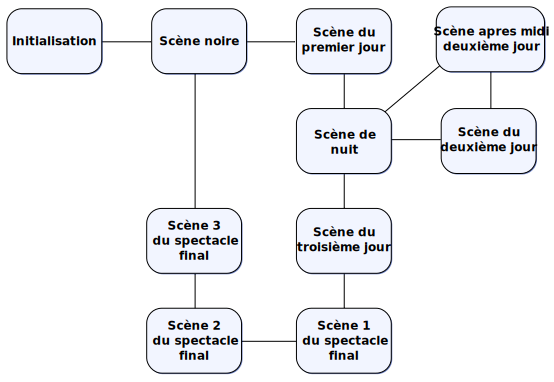
\includegraphics[width=\textwidth]{figs/scenario_complet_troisjours.pdf}
  \caption{Exemple d'un scénario complexe}
\end{figure}

\subsection{Les séries d'étapes}
Les séries d'étapes sont ce qui va décrire le fonctionnement de la carte à l'intérieur d'une scène. Dans chaque série d'étapes on trouve :
\begin{itemize}
\item Une étape de début (l'action d'initialisation de la scène)
\item Une étape de fin (l'action de sortie de la scène)
\item Aucune, une ou plusieurs étape(s) intermédiaire(s)
\item Aucune, une ou plusieurs transition(s)
\end{itemize}
\begin{figure}[htbp]
  \centering
  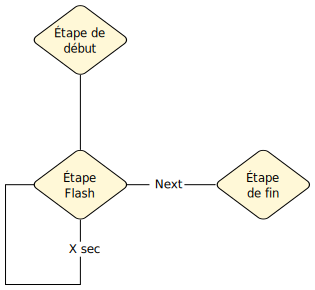
\includegraphics[width=.55\textwidth]{figs/etapes_simples.pdf}
  \caption{Série d'étapes simples}
  \label{fig:serie_etape_simple}
\end{figure}
La figure \ref{fig:serie_etape_simple} montre une série de taches toutes simples. Le fonctionnement de cet exemple sera détaillé plus loin, mais cette structure permet de faire clignoter une lumière toutes les $X$ secondes, $X$ étant défini auparavant.

\subsection{Les étapes}
Une étape est un élément très simple qui comporte un nom, un comportement de début d'étape et un comportement de fin d'étape.
Ce sont ces comportements qui font intervenir un langage textuel pour leur définition. L'utilisation d'un langage textuel et non un langage graphique sera argumenté plus tard.
\newpage
Voici un exemple d'étape :
\begin{figure}[htbp]
  \centering
  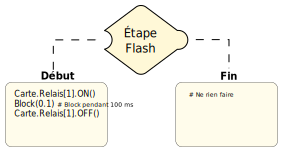
\includegraphics[width=.85\textwidth]{figs/etape_seule.pdf}
  \caption{Étape flash détaillée}
  \label{fig:etape_seule}
\end{figure} ~\\
Le code de début d'étape est rédigé dans une syntaxe simple, avec des actions toutes préparées. \\
Ici la première ligne permet de dire à la carte d'actionner sont premier relais. La seconde permet de bloquer le fonctionnement pendant 0.1 seconde, soit 100 millisecondes. La dernière permet d'éteindre le premier relais. \\
Ce qui est écrit en italic après le symbole \up{\textbf{\tiny \#}} sont des commentaires pour rendre le code encore plus compréhensible si besoin est.

\subsection{Les transitions}
Les transitions permettent de passer d'une étape à une autre ou encore d'une scène à une autre lorsque certaines conditions sont réunies.\p
Une transition attendra toujours que l'action de début d'une étape soit finie avant de faire quoi que ce soit. Ceci dans le but de ne pas provoquer de comportements chaotiques ou inattendus. Par exemple, dans l'étape flash présentée plus haut, si la transition \textit{Next} se déclenche alors que l'étape est sur sa seconde ligne, \textit{Block(0.1)}, le relais ne sera jamais éteins car la ligne suivante : \textit{Carte.Relais[1].OFF()} ne sera pas interprétée.\p
En revanche, les transitions entre scènes peuvent être déclenchées quelques soit l'étape en cours, tant que l'action de début d'étape est terminée évidemment.\p
Ensuite les transitions entre deux blocs (étape ou scène) sont forcément orientées de l'un à l'autre.\p
Enfin les transitions sont reliées à des signaux pour que celles-ci sachent quand il est utile de vérifier leur condition ou non, par exemple, un signal se déclenche dès qu'un ordre WIFI arrive, la transition qui attends l'ordre \textit{Next} va donc être lié à ce signal et vérifiera si l'ordre reçu est bien celui-ci, ou un autre.\p
Une transition ne pourra avoir que deux états, soit oui, soit non. Permettant dans le premier cas le franchissement de celle-ci et dans le second, laissant le scénario tel quel.\p
Voici un exemple de transition :
\begin{figure}[htbp]
  \centering
  \includegraphics[width=.80\textwidth]{figs/transition.pdf}
  \caption{Exemple de transition}
  \label{fig:transition}
\end{figure} ~\\

\subsection{Les interruptions}
Les interruptions permettent de garder une grande souplesse dans ce qu'il sera possible de faire via le système de scénario. En effet les étapes se déroulent dans une logique assez linéaire et les transitions ne sont franchies que si l'étape précédente est active. Comment alors perturber ce flux et par exemple mettre en pause tout le système sur un ordre WIFI, quel que soit l'étape en cours ?\p
Les interruptions sont là pour répondre à ce type de besoin. Une interruption est proche d'une transition, mais celle-ci peut :
\begin{itemize}
\item Être déclenchée, quelque soit l'étape en cours
\item Faire une action sans forcément changer l'étape en cours.
\end{itemize}~\\
Les interruptions sont elles aussi connectées à des signaux qui les réveillent. Une fois réveillées elles vérifient leur condition et si celle-ci est remplie elles exécutes des ordres définis.\p
Par exemple dans notre petite scène qui fait clignoter une lumière toutes les \textit{X} secondes, une interruption peut être utilisée pour changer cette valeur de \textit{X} en fonction d'un ordre reçu.
\begin{figure}[htbp]
  \centering
  \includegraphics[width=.95\textwidth]{figs/interruption.pdf}
  \caption{Exemple d'interruption}
  \label{fig:interruption}
\end{figure} ~\\

\section{Exemple d'application : Une poubelle intrigante}

Pour illustrer comment répondre à un besoin donné avec ce système de scénario voici un exemple concret.\\
Imaginons une poubelle qui possède un fonctionnement assez simple. Le jour elle joue une piste sonore en continue et grâce à un capteur de présence diminue le volume du son lorsque quelqu'un se rapproche et l'augmente lorsque celui-ci s'éloigne.\\
La nuit, la poubelle coasse\footnote{Du verbe coasser qui désigne le chant de la grenouille : \href{https://www.noslangues-ourlanguages.gc.ca/bien-well/fra-eng/vocabulaire-vocabulary/coasser-fra.html}{[lien]}} de temps à autres, et émet une lumière diffuse. Lorsque personne n'est a proximité la lumière est faible, mais lorsque quelqu'un s'approche celle-ci se met à briller de plus en plus.~\\
\indent Voyons comment il est possible de faire en sorte que la carte réponde à ce scénario.
\subsection{Le scénario}
Tout d'abord on peut identifier deux fonctionnements bien différents. L'un de journée, l'autre de soirée, il y aura donc deux scènes.\p
\begin{figure}[htbp]
  \centering
  \includegraphics[width=.90\textwidth]{figs/scenario_poubelle_scene.pdf}
  \caption{Scènes de l'exemple poubelle intrigantes}
  \label{fig:ex_poubelle_scene}
\end{figure} ~\\
En plus de la scène d'initialisation qui correspond au démarrage de la carte, nous avons bien deux scènes. Une pour le comportement de journée, l'autre pour celui de nuit. Les deux scènes sont liées par deux transitions, une dans chaque sens. Nous allons seulement en détailler une, l'autre étant presque identique.
\begin{figure}[htbp]
  \centering
  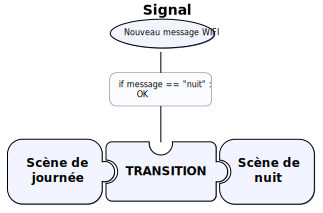
\includegraphics[width=0.65\textwidth]{figs/scenario_poubelle_scene_transition.pdf}
  \caption{Transition entre la scène de journée et la scène de nuit}
  \label{fig:ex_poubelle_scene_transition}
\end{figure} 

\newpage
\subsection{La scène de journée}
Nous allons détailler la série d'étapes de la scène de journée :
\begin{figure}[htbp]
  \centering
  \includegraphics[width=0.95\textwidth]{figs/etapes_poubelle_jour.pdf}
  \caption{Série d'étapes de la scène de journée}
  \label{fig:ex_poubelle_etapes_jour}
\end{figure} ~\\
Plusieurs choses sont intéressantes à remarquer ici : 
\begin{itemize}
\item Des transitions peuvent être sans condition, elles ne font qu'attendre que l'action de début de l'étape qui les précède soit finie.
\item Des étapes peuvent ne recevoir ou n'émettre aucune transition. Ici l'étape de fin est de toute façon jouée lorsque le scénario quitte la scène.
\item Une étape peut être vide de toute action. Ici l'étape d'attente est justement là pour attendre que le capteur de distance change de valeur et renvoyer soit sur l'étape qui monte le volume soit sur celle qui le descend. 
\end{itemize}\p
Nous allons maintenant détailler la transition \textit{Proche}, la transition \textit{Loin} étant très similaire.\newpage
\begin{figure}[htbp]
  \centering
  \includegraphics[width=0.85\textwidth]{figs/transition_poubelle.pdf}
  \caption{Transition entre l'étape d'attente et l'étape baisser le volume}
  \label{fig:ex_poubelle_transition_proche}
  \vspace{-25pt}
\end{figure} \p
Rien de surprenant, la transition attends que le signal \textit{Nouvelle valeur du capteur de distance} la réveille, vérifie que cette nouvelle valeur est bien inférieur à l'ancienne et si c'est le cas, déclenche le passage à l'étape \textit{Baisser le volume}.

\newpage
\subsection{La scène de nuit}
La scène de nuit est très similaire à la scène de journée, il suffit donc de reprendre la structure et d'en changer quelques éléments.\\
Voici à quoi ressemblerait la scène de nuit :
\begin{figure}[htbp]
  \centering
  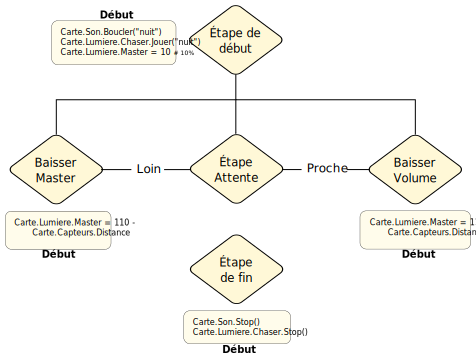
\includegraphics[width=0.95\textwidth]{figs/etapes_poubelle_nuit.pdf}
  \caption{Série d'étapes de la scène de nuit}
  \label{fig:ex_poubelle_etapes_nuit}
\end{figure} ~\\

\subsection{Les interruptions}
Aucune interruption n'est nécessaire pour ce scénario. En revanche on peut vouloir figer les poubelles pour que celles-ci ne fassent plus un bruit et n'émettent plus de lumière en leur ordonnant, puis leur permettre de reprendre leur fonctionnement.\p
Voici une proposition avec une interruption pour la pause, une autre pour reprendre le fonctionnement.
\newpage
\begin{figure}[htbp]
  \centering
  \includegraphics[width=0.95\textwidth]{figs/poubelle_interruption_pause.pdf}
  \caption{Interruption pour la mise en pause de la carte}
  \label{fig:ex_poubelle_interruption_pause}
  \vspace{-17pt}
\end{figure}
\begin{figure}[htbp]
  \centering
  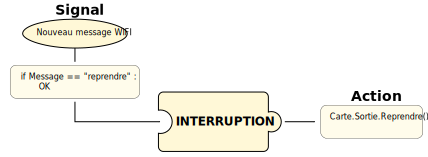
\includegraphics[width=0.95\textwidth]{figs/poubelle_interruption_resume.pdf}
  \caption{Interruption pour la reprise de la carte}
  \label{fig:ex_poubelle_interruption_resume}
\end{figure} ~\\
Les interruptions sont simples et permettent de perturber le flux sur un ordre WIFI directe.


\newpage
\section{Considérations techniques}
\indent \textit{Cette partie peut-être sautée par ce(lles)(ux) qui ne sont pas intéressé(e)s par les aspects purement technique du système}
\subsection{Latence du système de scénario}
Le système en lui même semble assez rapide sur le processeur Dragino. En effet la latence moyenne d'une interruption est de l'ordre de 2 ms. En imaginant qu'une interruption est souvent lié à un ordre il faut pour cela doubler ce temps. En rajoutant le traitement de l'information, même si celui-ci reste dans la majorité extrêmement simple, la plupart du temps une simple condition, pour obtenir une latence de l'ordre de 5 ms pour le système de scénario tournant sur le processeur Dragino.
\subsection{Latence de la communication Dragino-Atmega}
Il faut également considérer la latence due à la communication entre le processeur Dragino et la carte Atmega. Faute d'avoir pu réussir un essai directe je dois me fier aux informations trouvées sur le Web\footnote{\url{https://www.pjrc.com/teensy/td_libs_AltSoftSerial.html}}. Les taux de transfert pour de simples ordres semblent court : dans une fourchette comprise entre 0.1 ms et 5 ms en fonction des technologies utilisées. Majorons donc à 5 ms.
\subsection{Latence due au traitement de l'information de l'Atmega}
L'Atmega n'aura presque aucun calcul à faire, seulement à exécuter des ordres. Vu que la partie communication à déjà été prise en compte ci-dessus, je pense que l'on peut facilement prévoir des temps de réponses compris entre 1 et 5 ms en fonction de la tache à effectuer. Par exemple un \textit{chaser} sera beaucoup plus lourd à gérer que le déclenchement d'un flash.
\subsection{Latence due au réseau WIFI}
Cette latence sera la plus variable et aura comme principal paramètre l'état du réseau, la qualité des antennes et le nombre de bornes. Des essais que j'ai pu réaliser avec une seule borne, un réseau d'une qualité moyenne et une antenne peu adaptée j'obtiens une latence d'environs 2 ms. Avec plus de bornes et un signal moins bon je pense que cette latence peut atteindre entre 5 et 8 ms.
\subsection{Latence globale}
En réunissant toutes les latences majorées on obtiens un système avec un temps de réponse avoisinant les 20 ms ce qui semble un assez bon résultat. Pour s'en convaincre voici quelques ordres de grandeur :
\[ \text{Fréquence d'échantillonage de l'œil : } \]\[ f_{œil} \sim 25 \text{ Hz} \]\[
   \text{Période d'échantillonage de l'œil : } \]\[T_{œil} = \frac{1}{f_{œil}} \sim 40 \text{~ms}\]
   
	\[ \text{Vitesse du son dans le vide : }\]
	\[ v_{son} = 340 \text{~m.s\up{-1}} \]
	\[ \text{Temps de propagation du son dans le vide à 15 mètres} \]
	\[ t_{son} = \frac{15}{v_{son}} = 44 \text{~ms} \]

Sachant que la plupart de ces latences sont majorées et que tous les déclenchements ne passerons pas par le WIFI, le système pourra paraitre d'une bonne fluidité au yeux du public et des artistes.\\
De plus, pour les opérations demandant une synchronisation très poussée il sera possible de définir des \textit{latences tampons} permettant d'accuser les différents retards dues à la propagation des ordres et d'obtenir un déclenchement synchronisé avec une grande précision

\section{Choix et orientations}
\indent \textit{Une partie de cette section peut-être sautée par ce(lles)(ux) qui ne sont pas intéressé(e)s par les aspects purement technique du système}\p
Plusieurs choix dans cette propositions ont été fait sans contraintes particulières. Ce sont des cadres qui permettent de donner une forme au système et qui ont été motivés principalement par soucis de simplicité et de temps de développement. En revanche certains choix ont été fait par extrapolation et peuvent être erronés, c'est pourquoi je vais expliquer un petit peu plus ces choix, ce qui les a motivés pour qu'ils puissent être discutés et éventuellement changés.

\subsection{Un système pas 100\% graphique}
Le système de scénario sera en quelque sorte 90\% graphique et 10\% textuel. Pourquoi garder une petite partie en textuel et ne pas faire tout en graphique ?
\paragraph{Avantages}
\begin{itemize}
\item Pour la même souplesses dans les possibilités, une solution 100\% graphique demande un grand surcout en temps de développement par rapport au compromis de laisser une faible partie textuelle.
\item L'avantage du langage textuel est qu'il n'est pas figé et qu'il permet de pousser le système au delà de ses capacités prévues si besoin, sans pour autant modifier la structure de celui-ci.
\end{itemize}
\paragraph{Inconvénients}
\begin{itemize}
\item La partie textuelle demande la connaissance d'une syntaxe. Mais cette syntaxe est simple, assez réduite et sera fortement documentée.
\item Le plus gros désavantage que je vois est le fait que si il y a une faute de syntaxe (par exemple \textit{Carte.Lumier.Master} à la place de \textit{Carte.Lumiere.Master}) le système provoquera une erreur.
\end{itemize}

\subsection{Pas deux étapes actives en parallèle}
Le système sera prévue pour qu'il n'y ai toujours qu'une seule étape active.
\paragraph{Avantages}
\begin{itemize}
\item Cela réduit grandement les risques de comportements non souhaités, le parallélisme est toujours une grande source de problèmes.
\item Cela rend le système plus simple, au niveau de la création et de sa gestion. Il a donc de meilleures chances d'être plus réactif.
\end{itemize}
L'inconvénient pourrait être de se fermer beaucoup de possibilités car les cartes sont capables de faire du son, de la lumière, déclencher des actionneurs, etc et que de ne pas pouvoir en profiter serait dommage.\p
En réalité la carte Atmega sera capable de faire plusieurs actions en même temps et les étapes du scénario ne font que déclencher des événements qui ensuite pourront jouer en simultané. De plus le système d'interruption permet de créer un comportement pseudo-parallèle  au niveau des scénarios sans apporter de désavantages majeurs comme le parallélisme.

\subsection{Python comme langage de programmation}
Rien n'est fixé, mais je pense que python est le langage tout à fait adapté aux besoins du système.
\paragraph{Avantages}
\begin{itemize}
\item Souple et permet un développement rapide
\item Syntaxe claire et variables non typées ce qui permettra de rendre les 10\% de syntaxe comprit dans le système plus simple
\item La librairie Bridge du Yun Shield est écrite en Python !
\item C'est un langage que je maitrise bien et qui est simple à apprendre, ce qui réduira le temps de développement.
\end{itemize}
\paragraph{Inconvénient}
\begin{itemize}
\item Langage interprété donc forcément un peu plus lent que le C. Mais c'est un langage qui est très utilisé dans le calcul scientifique et qui est depuis devenu très mature. Il présente donc d'excellentes performances en générale.
\end{itemize}

\subsection{TCP comme protocole de transport selon le modèle OSI}
Le modèle OSI\footnote{\url{http://fr.wikipedia.org/wiki/Mod\%C3\%A8le_OSI\#Quelques_protocoles}} propose plusieurs protocoles pour le transport de l'information.\\
Je propose d'utiliser le protocole TCP pour cette fonction.
\paragraph{Avantages}
\begin{itemize}
\item Le protocole TCP permet de s'assurer qu'un message a bien été reçu et si n'est pas le cas le protocole se charge de le renvoyer. On a donc quelque chose de robuste et la quasi certitude que chaque ordre sera reçu.
\item Le protocole TCP est plus simple à mettre en place, plus utilisé et plus robuste de manière générale (il évite de surcharger le réseau lorsque celui-ci est saturé etc.)
\item Le protocole TCP est intègre. Il s'assure que les données n'ont pas été corrompues pendant le transfert, on ne risque pas d'avoir un ordre Y reçu pour un ordre X envoyé.
\end{itemize}
\paragraph{Inconvénient}
\begin{itemize}
\item Le protocole TCP est plus lent que le protocole UDP en général. En revanche il ne présente pas d'énormes latence pour un réseau comme le notre et surtout permet dans de nombreux cas d'être plus rapide que l'UDP de part sa bonne gestion du réseau\footnote{\url{http://stackoverflow.com/questions/47903/udp-vs-tcp-how-much-faster-is-it}}. Cela reste tout de même à vérifier sur des tests à plus grande échelle.
\end{itemize}


\section{Conclusion}
Ce document a donc essayé de présenter le plus clairement possible une solution pour le système de scénario. Cette solution est bien évidement une proposition, et pleins de choses restes à définir. En revanche c'est une proposition qui est techniquement viable et j'ai déjà fait plusieurs essais de code pour tester cette logique d'interruption de transition et d'autres concepts mis ne jeu par le système présenté.\p
Pour que je puisse avancer au plus vite sans non plus me lancer dans une direction qui ne serait pas la bonne il me faut donc savoir si ce système, aux modifications prêt évidement, correspond bien aux attentes du projet.



   
   



\end{document}